\documentclass[fleqn,xcolor=table,10pt,final]{beamer}

\setbeamertemplate{footline}[text line]{%
    \parbox{\linewidth}{\vspace*{-8pt}
    \tt{https://github.com/AlbertDeFusco/goldRush}
  \hfill}}
\setbeamertemplate{navigation symbols}{}
\usepackage{amsmath,amsfonts,amssymb,pxfonts,xspace}
\usepackage{textpos}
\usepackage{colortbl}
\usepackage{verbatim}
\usepackage{graphicx}
\usepackage{color}
\usepackage{listings}
\usepackage{tikz}

\definecolor{green}{rgb}{0.1,0.8,0.1}
\definecolor{gold}{rgb}{0.85,.66,0}

\lstset{
    basicstyle=\footnotesize,
    keywordstyle=\color[rgb]{0.1,0.8,0.1}\bfseries,
    commentstyle=\color{blue},
    numbers=left,
    stringstyle=\ttfamily\color{red!50!brown},
    showstringspaces=false}
\lstset{literate=%
   *{0}{{{\color{red!20!violet}0}}}1
    {1}{{{\color{red!20!violet}1}}}1
    {2}{{{\color{red!20!violet}2}}}1
    {3}{{{\color{red!20!violet}3}}}1
    {4}{{{\color{red!20!violet}4}}}1
    {5}{{{\color{red!20!violet}5}}}1
    {6}{{{\color{red!20!violet}6}}}1
    {7}{{{\color{red!20!violet}7}}}1
    {8}{{{\color{red!20!violet}8}}}1
    {9}{{{\color{red!20!violet}9}}}1
}



\begin{document}

\title{Cilk Plus Reducers}
\author{Albert DeFusco}
\date{\today}
\frame{\titlepage}


\begin{frame}
  \frametitle{Parallel Gold Sifting}
  \begin{itemize}
    \item Each pan can sift a constant amount of dirt/day
    \item More pans means more dirt sifted
  \end{itemize}
  \vskip 0.2cm
  \begin{itemize}
    \item<2-> Each pan sifts independently
    \item<2-> Each pan has a defined amount of dirt to sift
  \end{itemize}
  \vskip 0.2cm
  \begin{itemize}
    \item<3-> Sifting is parallelizable
  \end{itemize}
\end{frame}

\begin{frame}[fragile]
  \frametitle{Serial Gold Sifting}
  \begin{lstlisting}[language=C++,basicstyle=\scriptsize]
#include <list>
class pan
{
  public:
    pan();          //create array of random integers between 1 and 10,000
    int sift();     //returns frequency of the number 79 (atomic number of gold)
    bool hasGold(); //calls sift; returns true if sift() > 0
}

int main()
{
  std::list<int> withGold;
  Pan* myPans = new Pan[nPans];

  for(int i=0; i<nPans; ++i)
  {
    bool gold = myPans[i].hasGold();
    if(gold) {
      withGold.push_back(i);
    }
  }
  std::list<int>::const_iterator iterator;
  for (iterator = withGold.begin(); iterator != withGold.end(); ++iterator)
    std::cout << *iterator << "  ";
  std::cout << endl;

  return 0;
}
  \end{lstlisting}
\end{frame}

\begin{frame}[fragile]
  \frametitle{Gold Rush}
  {\scriptsize
  \begin{verbatim}
Gold Rush!

  10000 total chunks of dirt
  1000 pans

  Found gold in 15 pans
  Pan IDs: 94  142  265  268  289  440  442  443  569  600  721  781  783  806  818

serial execution took 5.60495 seconds
  \end{verbatim}
}
\end{frame}


\begin{frame}[fragile]
  \frametitle{Parallel Gold Sifting}
  \begin{lstlisting}[language=C++,basicstyle=\scriptsize]
#include <list>
#include <cilk/cilk.h>
class pan
{
  public:
    pan();          //create array of random integers between 1 and 10,000
    int sift();     //returns frequency of the number 79 (atomic number of gold)
    bool hasGold(); //calls sift; returns true if sift() > 0
}

int main()
{
  std::list<int> withGold;
  Pan* myPans = new Pan[nPans];

  cilk_for(int i=0; i<nPans; ++i)
  {
    bool gold = myPans[i].hasGold();
    if(gold) {
      withGold.push_back(i);
    }
  }
  std::list<int>::const_iterator iterator;
  for (iterator = withGold.begin(); iterator != withGold.end(); ++iterator)
    std::cout << *iterator << "  ";
  std::cout << endl;

  return 0;
}
  \end{lstlisting}
  \begin{tikzpicture}[overlay]
    \draw[color=red] (5.5,2.4) rectangle (0.0,4.4);
  \end{tikzpicture}
\end{frame}

\begin{frame}
  \frametitle{Parallel Gold Sifting}
  \begin{itemize}
    \item There is a problem to be solved
      \begin{itemize}
        \item How do we keep track of which pans have gold?
      \end{itemize}
      \vskip 1.0cm
    \item Where does the result get stored?
    \item Who can access the result?
  \end{itemize}
\end{frame}

\begin{frame}[fragile]
  \frametitle{Parallel Gold Sifting}
  \begin{lstlisting}[language=C++,basicstyle=\scriptsize]
#include <list>
#include <cilk/cilk.h>
class pan
{
  public:
    pan();          //create array of random integers between 1 and 10,000
    int sift();     //returns frequency of the number 79 (atomic number of gold)
    bool hasGold(); //calls sift; returns true if sift() > 0
}

int main()
{
  std::list<int> withGold;
  Pan* myPans = new Pan[nPans];

  cilk_for(int i=0; i<nPans; ++i)
  {
    bool gold = myPans[i].hasGold();
    if(gold) {
      withGold.push_back(i);
    }
  }
  std::list<int>::const_iterator iterator;
  for (iterator = withGold.begin(); iterator != withGold.end(); ++iterator)
    std::cout << *iterator << "  ";
  std::cout << endl;

  return 0;
}
  \end{lstlisting}
  \begin{tikzpicture}[overlay]
    \draw[color=red] (5.5,2.5) rectangle (0.0,4.5);
    %\draw[color=blue] (6,2.5) rectangle (10,4.5);
    \node[draw,align=center] at (8,3.5) {\color{red} may not be thread-safe};
    %\item It is inefficient to hire a foreman to just count gold
  \end{tikzpicture}
\end{frame}


\begin{frame}
  \frametitle{Thread Safety}
  \begin{itemize}
    \item Unsafe operations
      \begin{itemize}
        \item Multiple threads accessing the same address
          \begin{itemize}
            \item Basic types are not thread safe
            \item STL containers \emph{may} be thread safe for some operations
          \end{itemize}
      \end{itemize}
    \itemsep 0.5cm
    \item<2-> Threads read and write memory at undetermined times
    \item<3-> Leads to a race condition
  \end{itemize}
\end{frame}

\begin{frame}
  \frametitle{Race Condition}
  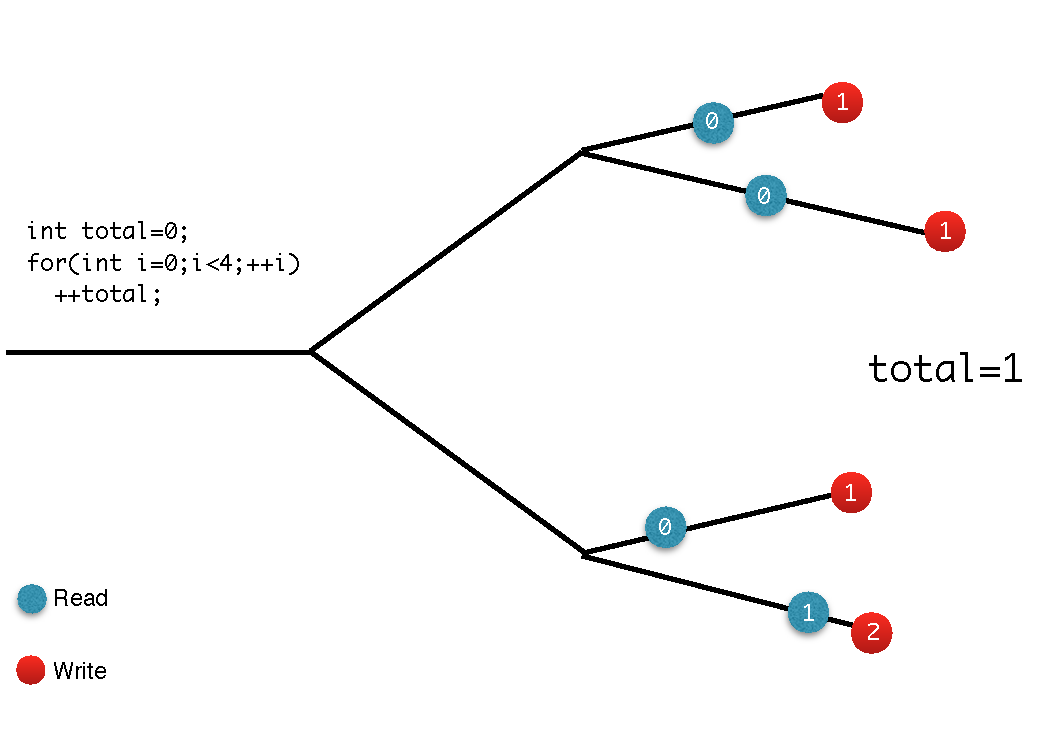
\includegraphics[width=\textwidth]{figures/race}
\end{frame}

\begin{frame}[fragile]
  \frametitle{Inefficient solutions}
  \begin{itemize}
    \itemsep 0.4cm
    \item Locking
      \begin{itemize}
        \item Requires careful programming
        \item Non deterministic
      \end{itemize}
    \item cannot use {\tt cilk\_sync} in the loop
      \begin{itemize}
        \item will only sync child threads, not all threads
      \end{itemize}
    \item Break the loop
      \begin{itemize}
        \item Requires more storage and management
      \end{itemize}
  \end{itemize}
  \begin{lstlisting}[language=C++,basicstyle=\scriptsize]
#include <cilk/cilk.h>

double *sum = new double[N];
//parallel
cilk_for(int i=0;i<N;++i)
  sum[N] = f(N);

//serial
double total=0.0;
for(int i=0;i<N;++i)
  total+=sum[N];
  \end{lstlisting}
\end{frame}

\begin{frame}
  \frametitle{Cilk Reducers}
  \begin{itemize}
    \item Provide thread safe access to a ``smart pointer''
    \item Any associative operation is a valid reducer
      \begin{equation*}
        x\ OP\ y = y\ OP\ x
      \end{equation*}
    \item Small performance overhead for usage
    \item Very extensible in C++
    \item Operations are guaranteed to execute in the same order as in serial
  \end{itemize}
\end{frame}

\begin{frame}[fragile]
  \frametitle{Cilk Reducers: views}
  \begin{lstlisting}[language=C++,basicstyle=\scriptsize]
#include <cilk/reducer_opadd.h>
int total=0;
cilk::reducer<cilk::<op_add<int>> reducer_total (0);
for(int i=0;i<4;++i)
  ++*reducer_total;
total = reducer_total.get_value();
  \end{lstlisting}
  \begin{itemize}
    \item At spawn each strand gets a private \emph{view} of the reducer
    \item When strands merge
      \begin{itemize}
        \item \emph{views} are combined by $OP$
        \item The combined \emph{view} is given to the exit strand
      \end{itemize}
  \end{itemize}
\end{frame}

\begin{frame}
  \frametitle{Cilk Reducers: views}
  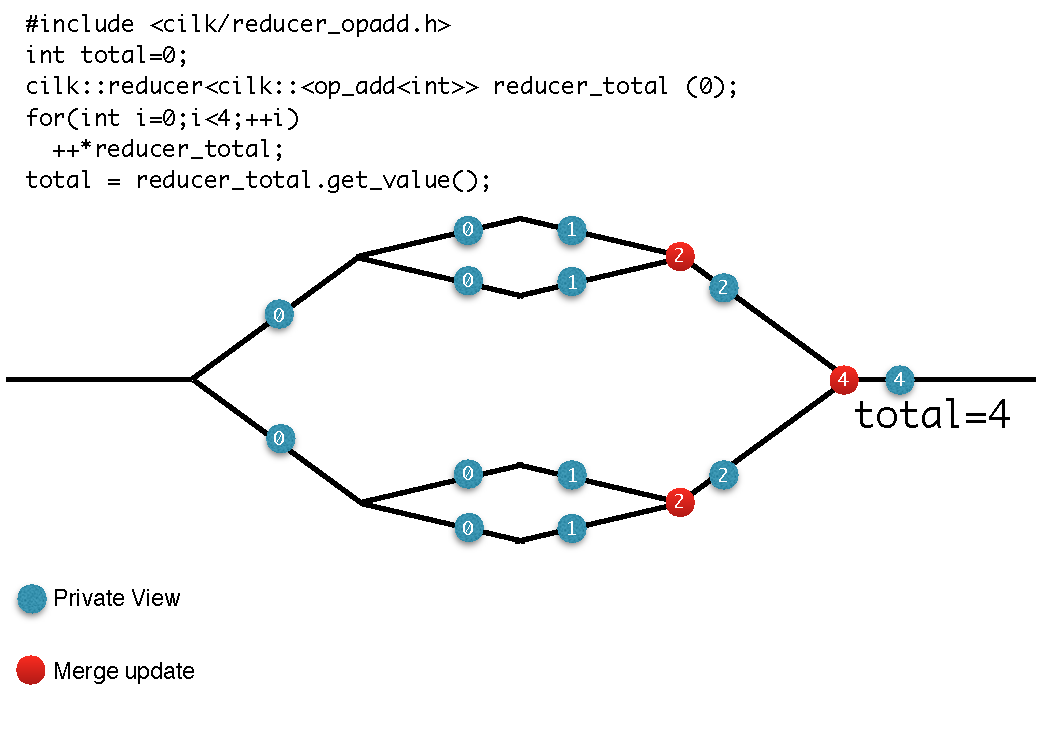
\includegraphics[width=\textwidth]{figures/reduce}
\end{frame}

\begin{frame}[fragile]
  \frametitle{Cilk Reducers: types}
    {\scriptsize
  usage: \verb|cilk::reducer<cilk::REDUCER_TYPE<<my_type>> my_reducer;|
  \begin{table}
    \begin{tabular}{l|c|l}
      Reducer Type & Description & Header\\
      \hline
      \tt{op\_add} & \tt{++, --, +=, -=, +, -} & \verb|#include <cilk/reducer_add.h>|\\
      \tt{op\_vector} & Provides \verb|push_back()|& \verb|#include <cilk/reducer_vector.h>|\\
      \tt{op\_list\_append} & Provides \verb|push_back()|& \verb|#include <cilk/reducer_list.h>|\\
      \tt{op\_list\_prepend} & Provides \verb|push_front()|& \verb|#include <cilk/reducer_list.h>|\\
      \tt{op\_max} & Returns maximum & \verb|#include <cilk/reducer_max.h>|\\
      \tt{op\_min} & Returns minimum & \verb|#include <cilk/reducer_min.h>|\\
      \tt{op\_ostream} & Provides \tt{<<}& \verb|#include <cilk/reducer_string.h>|
    \end{tabular}
    \caption{\tt{https://software.intel.com/en-us/node/522606}}
  \end{table}
}

\end{frame}


\begin{frame}[fragile]
  \frametitle{Parallel gold sifting}
  \begin{lstlisting}[language=C++,basicstyle=\scriptsize]
#include <cilk/cilk.h>
#include <cilk/reducer_list.h>

  std::list<int> withGold;
  cilk::reducer< cilk::op_list_append<int> > reducer_withGold;
  Pan* myPans = new Pan[nPans];

  cilk_for(int i=0; i<nPans; ++i)
  {
    bool gold = myPans[i].hasGold();
    if(gold) {
      reducer_withGold->push_back(i);
    }
  }
  withGold = reducer_withGold.get_value();

  std::list<int>::const_iterator iterator;
  for (iterator = withGold.begin(); iterator != withGold.end(); ++iterator)
    std::cout << *iterator << "  ";
  std::cout << endl;
  \end{lstlisting}
  \begin{tikzpicture}[overlay]
    \draw[color=blue] (0.2,4.8) rectangle (9.3,5.1);
    \draw[color=blue] (0.8,2.8) rectangle (5.5,3.1);
    \draw[color=blue] (0.3,2) rectangle (6.2,2.3);
  \end{tikzpicture}
\end{frame}

\begin{frame}[fragile]
  \frametitle{Gold Rush}
  {\scriptsize
  \begin{verbatim}
$>cat /proc/cpuinfo | grep Xeon | uniq -c
     16 model name      : Intel(R) Xeon(R) CPU E5-2670 0 @ 2.60GHz
$>CILK_NWORKERS=16 ./goldRush
Gold Rush!

  100000 total chunks of dirt
  1000 pans

  Found gold in 15 pans
  Pan IDs: 94  142  265  268  289  440  442  443  569  600  721  781  783  806  818

Cilk identified the correct pans

serial execution took 5.60154 seconds

parallel execution took 0.39801 seconds with 16 workers
parallel speedup 14.0739
paralell efficiency 0.879616
  \end{verbatim}
}
\end{frame}

\end{document}
